\documentclass{article}

\usepackage[margin=1in]{geometry}
\usepackage[utf8]{inputenc}
\usepackage{amsmath}
\usepackage{tikz}
\usepackage{sectsty}
\usetikzlibrary{automata,positioning}

\title{Homework \#1}
\date{April 7th 2020}
\author{Zohreh Sadeghi,\\University of Washington, Tacoma}

\sectionfont{\fontsize{12}{15}\selectfont}

\begin{document}

\maketitle

\section{Problem 1}

\paragraph{Part a}$\{ w | w \textrm{ begins with } 01 \wedge w \textrm{ ends with } 0 \}$

\begin{center}
    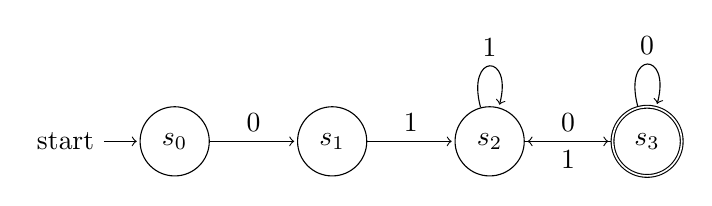
\begin{tikzpicture}[shorten >=1pt,node distance=2cm,on grid,auto] 
        \node[state,initial] (s_0)   {$s_0$}; 
        \node[state] (s_1) [right=of s_0] {$s_1$}; 
        \node[state] (s_2) [right=of s_1] {$s_2$}; 
        \node[state,accepting](s_3) [right=of s_2] {$s_3$};
        \path[->] 
        (s_0) edge node {0} (s_1)
        (s_1) edge node {1} (s_2)
        (s_2) edge node {0} (s_3)
        edge [loop above] node {1} ()
        (s_3) edge node {1} (s_2)
        edge [loop above] node {0} ();
    \end{tikzpicture}
\end{center}

\paragraph{Part b}$\{ w | \{0,1\}^\ast-\{01,001\} \}$

\begin{center}
    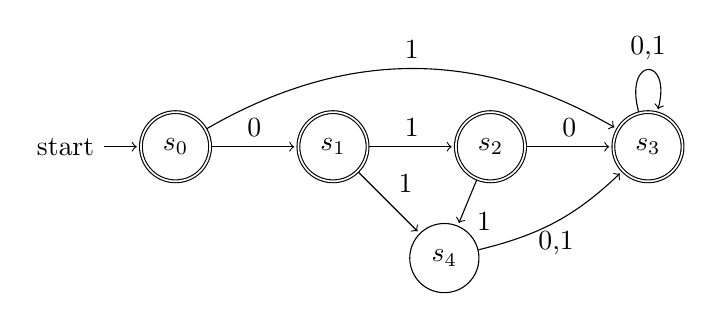
\begin{tikzpicture}[shorten >=1pt,node distance=2cm,on grid,auto] 
        \node[state,initial,accepting] (s_0)   {$s_0$}; 
        \node[state,accepting] (s_1) [right=of s_0] {$s_1$}; 
        \node[state,accepting] (s_2) [right=of s_1] {$s_2$}; 
        \node[state,accepting] (s_3) [right=of s_2] {$s_3$};
        \node[state] (s_4) [below right=of s_1] {$s_4$};
        \path[->] 
        (s_0) edge node {0} (s_1)
        edge[bend left=30] node {1} (s_3)
        
        (s_1) edge node {1} (s_2)
        edge node {1} (s_4)
        
        (s_2) edge node {0} (s_3)
        edge node {1} (s_4)
        
        (s_3) edge [loop above] node {0,1} ()
        
        (s_4) edge[bend right=15] node[anchor=north] {0,1} (s_3);
    \end{tikzpicture}
\end{center}

\paragraph{Part c}$\{ w | \textrm{even positions of } w \textrm{ are } 1 \}$

\begin{center}
    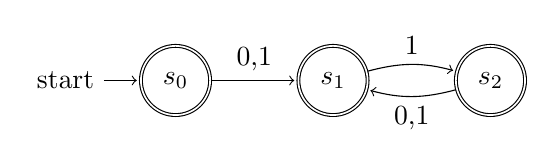
\begin{tikzpicture}[shorten >=1pt,node distance=2cm,on grid,auto] 
        \node[state,initial,accepting] (s_0)   {$s_0$}; 
        \node[state,accepting] (s_1) [right=of s_0] {$s_1$}; 
        \node[state,accepting] (s_2) [right=of s_1] {$s_2$}; 
        \path[->] 
        (s_0) edge node {0,1} (s_1)
        (s_1) edge[bend left=15] node[anchor=south] {1} (s_2)
        (s_2) edge[bend left=15] node[anchor=north] {0,1} (s_1);
    \end{tikzpicture}
\end{center}

\paragraph{Part d}$\{ w | w \textrm{contains an even number of } 1 \wedge w \textrm{ has at most two } 0 \}$

\begin{center}
    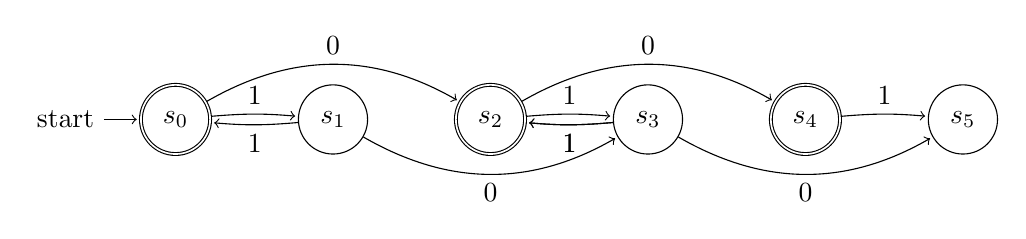
\begin{tikzpicture}[shorten >=1pt,node distance=2cm,on grid,auto] 
        \node[state,initial,accepting] (s_0)   {$s_0$}; 
        \node[state] (s_1) [right=of s_0] {$s_1$}; 
        \node[state,accepting] (s_2) [right=of s_1] {$s_2$}; 
        \node[state] (s_3) [right=of s_2] {$s_3$}; 
        \node[state,accepting] (s_4) [right=of s_3] {$s_4$}; 
        \node[state] (s_5) [right=of s_4] {$s_5$}; 
        \path[->] 
        (s_0) edge[bend left=5] node[anchor=south] {1} (s_1)
        edge[bend left] node {0} (s_2)
        (s_1) edge[bend left=5] node[anchor=north] {1} (s_0)
        edge[bend right] node[anchor=north] {0} (s_3)
        (s_2) edge[bend left=5] node[anchor=south] {1} (s_3)
        edge[bend left] node {0} (s_4)
        (s_3) edge[bend left=5] node[anchor=north] {1} (s_2)
        edge[bend right] node[anchor=north] {0} (s_5)
        (s_4) edge[bend left=5] node[anchor=south] {1} (s_5)
        (s_3) edge[bend left=5] node[anchor=north] {1} (s_2)
        ;
    \end{tikzpicture}
\end{center}

\section{Problem 2}

\paragraph{Part a} $L=\{ w | |w| \bmod 2 = 1 \wedge \textrm{ number of b's is even} \}$

\paragraph{Length is odd}

\begin{center}
    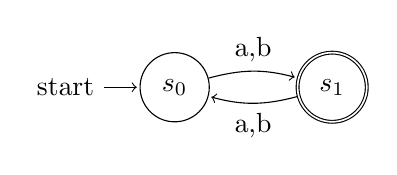
\begin{tikzpicture}[shorten >=1pt,node distance=2cm,on grid,auto] 
        \node[state,initial] (s_0)   {$s_0$}; 
        \node[state,accepting] (s_1) [right=of s_0] {$s_1$}; 
        \path[->] 
        (s_0) edge[bend left=15] node[anchor=south] {a,b} (s_1)
        (s_1) edge[bend left=15] node[anchor=north] {a,b} (s_0);
    \end{tikzpicture}
\end{center}

Where the language $M_1$ defining the above DFA can be written as:

\begin{align*}
& M_1=\left( Q_1, \Sigma_1, \delta_1, q_0', F_1 \right) \\
& Q_1=\{ s_0, s_1 \} \\
& \Sigma_1=\{ a, b \} \\
& \delta_1=\begin{cases}
    s_0 &r_i=s_1 \\
    s_1 &r_i=s_0
\end{cases} \\
& q_0'=s_0 \\
& F_1=\{ s_1 \}
\end{align*}

\paragraph{Has an even number of $b$s}

\begin{center}
    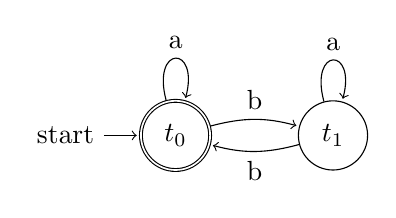
\begin{tikzpicture}[shorten >=1pt,node distance=2cm,on grid,auto] 
        \node[state,initial, accepting] (s_0)   {$t_0$}; 
        \node[state] (s_1) [right=of s_0] {$t_1$}; 
        \path[->] 
        (s_0) edge[bend left=15] node[anchor=south] {b} (s_1)
        edge [loop above] node {a} ()
        (s_1) edge[bend left=15] node[anchor=north] {b} (s_0)
        edge [loop above] node {a} ();
    \end{tikzpicture}
\end{center}

Where the language $M_2$ defining the above DFA can be written as:

\begin{align*}
& M_2=\left( Q_2, \Sigma_2, \delta_2, q_0", F_2 \right) \\
& Q_2=\{ t_0, t_1 \} \\
& \Sigma_2=\{ a, b \} \\
& \delta_2=\begin{cases}
    t_0 &r_i=t_1 \wedge w_{i+1}=b \\
    t_1 &r_i=t_0 \wedge w_{i+1}=b \\
    r_i &\textrm{otherwise}
\end{cases} \\
& q_0"=t_0 \\
& F_2=\{ t_0 \}
\end{align*}

\paragraph{Part b} Give the formal description of your DFAs.\\

Language $L=M_1\cap{}M_2$ can be defined as:

\begin{align*}
& L=\left( Q, \Sigma, \delta, q_0, F \right) \\
& Q= Q_1 \times Q_2 = \{ (s_0,t_0),(s_0,t_1),(s_1,t_0),(s_1,t_1) \} \\
& \Sigma{}=\Sigma_1=\Sigma_2=\{ a, b \} \\
& \delta\left( (r_i',r_i"), w_{i+1} \right)=\left( \delta_1(r_i',w_{i+1}), \delta_2(r_i", w_{i+1}) \right) \\
& q_0=(s_0,t_0) \\
& F_2=\{ (s_1,t_0) \}
\end{align*}

And the diagram would be:


\begin{center}
    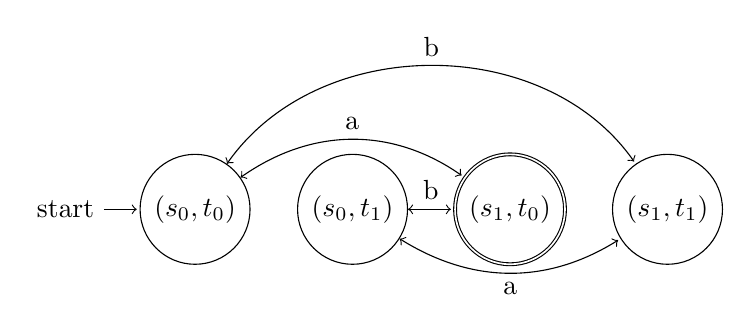
\begin{tikzpicture}[shorten >=1pt,node distance=2cm,on grid,auto,every edge/.append style={<->}] 
        \node[state,initial] (z_0)   {$(s_0,t_0)$}; 
        \node[state] (z_1) [right=of z_0] {$(s_0,t_1)$}; 
        \node[state, accepting] (z_2) [right=of z_1] {$(s_1,t_0)$}; 
        \node[state] (z_3) [right=of z_2] {$(s_1,t_1)$}; 
        \path[->] 
        (z_0) edge[bend left=35] node[anchor=south] {a} (z_2)
        edge[bend left=55] node[anchor=south] {b} (z_3)
        (z_1) edge node {b} (z_2)
        edge[bend right=32] node[anchor=north] {a} (z_3)
        ;
    \end{tikzpicture}
\end{center}

\section{Problem 3}

\paragraph{Part b}

This DFA describes a language where all words have a substring that matches the pattern where we have one or more $0$s, followed by
one or more $1$s, followed by at least one $0$. All the other characters before and after this pattern are immaterial.

\begin{equation*}
    L = \{ w | \textrm{ w contains } 00^\ast11^\ast0 \}
\end{equation*}


\end{document}  
